\documentclass[twoside]{book}

% Packages required by doxygen
\usepackage{fixltx2e}
\usepackage{calc}
\usepackage{doxygen}
\usepackage[export]{adjustbox} % also loads graphicx
\usepackage{graphicx}
\usepackage[utf8]{inputenc}
\usepackage{makeidx}
\usepackage{multicol}
\usepackage{multirow}
\PassOptionsToPackage{warn}{textcomp}
\usepackage{textcomp}
\usepackage[nointegrals]{wasysym}
\usepackage[table]{xcolor}

% NLS support packages
\usepackage[french]{babel}

% Font selection
\usepackage[T1]{fontenc}
\usepackage[scaled=.90]{helvet}
\usepackage{courier}
\usepackage{amssymb}
\usepackage{sectsty}
\renewcommand{\familydefault}{\sfdefault}
\allsectionsfont{%
  \fontseries{bc}\selectfont%
  \color{darkgray}%
}
\renewcommand{\DoxyLabelFont}{%
  \fontseries{bc}\selectfont%
  \color{darkgray}%
}
\newcommand{\+}{\discretionary{\mbox{\scriptsize$\hookleftarrow$}}{}{}}

% Page & text layout
\usepackage{geometry}
\geometry{%
  a4paper,%
  top=2.5cm,%
  bottom=2.5cm,%
  left=2.5cm,%
  right=2.5cm%
}
\tolerance=750
\hfuzz=15pt
\hbadness=750
\setlength{\emergencystretch}{15pt}
\setlength{\parindent}{0cm}
\setlength{\parskip}{3ex plus 2ex minus 2ex}
\makeatletter
\renewcommand{\paragraph}{%
  \@startsection{paragraph}{4}{0ex}{-1.0ex}{1.0ex}{%
    \normalfont\normalsize\bfseries\SS@parafont%
  }%
}
\renewcommand{\subparagraph}{%
  \@startsection{subparagraph}{5}{0ex}{-1.0ex}{1.0ex}{%
    \normalfont\normalsize\bfseries\SS@subparafont%
  }%
}
\makeatother

% Headers & footers
\usepackage{fancyhdr}
\pagestyle{fancyplain}
\fancyhead[LE]{\fancyplain{}{\bfseries\thepage}}
\fancyhead[CE]{\fancyplain{}{}}
\fancyhead[RE]{\fancyplain{}{\bfseries\leftmark}}
\fancyhead[LO]{\fancyplain{}{\bfseries\rightmark}}
\fancyhead[CO]{\fancyplain{}{}}
\fancyhead[RO]{\fancyplain{}{\bfseries\thepage}}
\fancyfoot[LE]{\fancyplain{}{}}
\fancyfoot[CE]{\fancyplain{}{}}
\fancyfoot[RE]{\fancyplain{}{\bfseries\scriptsize Généré par Doxygen }}
\fancyfoot[LO]{\fancyplain{}{\bfseries\scriptsize Généré par Doxygen }}
\fancyfoot[CO]{\fancyplain{}{}}
\fancyfoot[RO]{\fancyplain{}{}}
\renewcommand{\footrulewidth}{0.4pt}
\renewcommand{\chaptermark}[1]{%
  \markboth{#1}{}%
}
\renewcommand{\sectionmark}[1]{%
  \markright{\thesection\ #1}%
}

% Indices & bibliography
\usepackage{natbib}
\usepackage[titles]{tocloft}
\setcounter{tocdepth}{3}
\setcounter{secnumdepth}{5}
\makeindex

% Hyperlinks (required, but should be loaded last)
\usepackage{ifpdf}
\ifpdf
  \usepackage[pdftex,pagebackref=true]{hyperref}
\else
  \usepackage[ps2pdf,pagebackref=true]{hyperref}
\fi
\hypersetup{%
  colorlinks=true,%
  linkcolor=blue,%
  citecolor=blue,%
  unicode%
}

% Custom commands
\newcommand{\clearemptydoublepage}{%
  \newpage{\pagestyle{empty}\cleardoublepage}%
}

\usepackage{caption}
\captionsetup{labelsep=space,justification=centering,font={bf},singlelinecheck=off,skip=4pt,position=top}

%===== C O N T E N T S =====

\begin{document}

% Titlepage & ToC
\hypersetup{pageanchor=false,
             bookmarksnumbered=true,
             pdfencoding=unicode
            }
\pagenumbering{alph}
\begin{titlepage}
\vspace*{7cm}
\begin{center}%
{\Large Medi\+Watch\+Web\+Site \\[1ex]\large 0.\+0.\+0-\/\+M\+VP }\\
\vspace*{1cm}
{\large Généré par Doxygen 1.8.13}\\
\end{center}
\end{titlepage}
\clearemptydoublepage
\pagenumbering{roman}
\tableofcontents
\clearemptydoublepage
\pagenumbering{arabic}
\hypersetup{pageanchor=true}

%--- Begin generated contents ---
\chapter{Index des espaces de nommage}
\doxysection{Liste des espaces de nommage}
Liste de tous les espaces de nommage documentés avec une brève description\+:\begin{DoxyCompactList}
\item\contentsline{section}{\mbox{\hyperlink{namespace_blazing_blog}{Blazing\+Blog}} }{\pageref{namespace_blazing_blog}}{}
\item\contentsline{section}{\mbox{\hyperlink{namespace_blazing_blog_1_1_server}{Blazing\+Blog.\+Server}} }{\pageref{namespace_blazing_blog_1_1_server}}{}
\item\contentsline{section}{\mbox{\hyperlink{namespace_blazing_blog_1_1_server_1_1_controllers}{Blazing\+Blog.\+Server.\+Controllers}} }{\pageref{namespace_blazing_blog_1_1_server_1_1_controllers}}{}
\item\contentsline{section}{\mbox{\hyperlink{namespace_mediwatch}{Mediwatch}} }{\pageref{namespace_mediwatch}}{}
\item\contentsline{section}{\mbox{\hyperlink{namespace_mediwatch_1_1_server}{Mediwatch.\+Server}} }{\pageref{namespace_mediwatch_1_1_server}}{}
\item\contentsline{section}{\mbox{\hyperlink{namespace_mediwatch_1_1_server_1_1_areas}{Mediwatch.\+Server.\+Areas}} }{\pageref{namespace_mediwatch_1_1_server_1_1_areas}}{}
\item\contentsline{section}{\mbox{\hyperlink{namespace_mediwatch_1_1_server_1_1_areas_1_1_identity}{Mediwatch.\+Server.\+Areas.\+Identity}} }{\pageref{namespace_mediwatch_1_1_server_1_1_areas_1_1_identity}}{}
\item\contentsline{section}{\mbox{\hyperlink{namespace_mediwatch_1_1_server_1_1_areas_1_1_identity_1_1_data}{Mediwatch.\+Server.\+Areas.\+Identity.\+Data}} }{\pageref{namespace_mediwatch_1_1_server_1_1_areas_1_1_identity_1_1_data}}{}
\item\contentsline{section}{\mbox{\hyperlink{namespace_mediwatch_1_1_server_1_1_controllers}{Mediwatch.\+Server.\+Controllers}} \\*Test controller }{\pageref{namespace_mediwatch_1_1_server_1_1_controllers}}{}
\item\contentsline{section}{\mbox{\hyperlink{namespace_mediwatch_1_1_server_1_1_migrations}{Mediwatch.\+Server.\+Migrations}} }{\pageref{namespace_mediwatch_1_1_server_1_1_migrations}}{}
\item\contentsline{section}{\mbox{\hyperlink{namespace_mediwatch_1_1_server_1_1_migrations_1_1_db_context_mediwatch_migrations}{Mediwatch.\+Server.\+Migrations.\+Db\+Context\+Mediwatch\+Migrations}} }{\pageref{namespace_mediwatch_1_1_server_1_1_migrations_1_1_db_context_mediwatch_migrations}}{}
\item\contentsline{section}{\mbox{\hyperlink{namespace_mediwatch_1_1_server_1_1_pages}{Mediwatch.\+Server.\+Pages}} }{\pageref{namespace_mediwatch_1_1_server_1_1_pages}}{}
\item\contentsline{section}{\mbox{\hyperlink{namespace_mediwatch_1_1_server_1_1_ressources}{Mediwatch.\+Server.\+Ressources}} }{\pageref{namespace_mediwatch_1_1_server_1_1_ressources}}{}
\item\contentsline{section}{\mbox{\hyperlink{namespace_server}{Server}} }{\pageref{namespace_server}}{}
\item\contentsline{section}{\mbox{\hyperlink{namespace_server_1_1_utils}{Server.\+Utils}} }{\pageref{namespace_server_1_1_utils}}{}
\end{DoxyCompactList}

\chapter{Index hiérarchique}
\section{Hiérarchie des classes}
Cette liste d\textquotesingle{}héritage est classée approximativement par ordre alphabétique \+:\begin{DoxyCompactList}
\item Controller\begin{DoxyCompactList}
\item \contentsline{section}{Mediwatch.\+Server.\+Controllers.\+Email\+Controller}{\pageref{class_mediwatch_1_1_server_1_1_controllers_1_1_email_controller}}{}
\end{DoxyCompactList}
\item Controller\+Base\begin{DoxyCompactList}
\item \contentsline{section}{Blazing\+Blog.\+Server.\+Controllers.\+Articles\+Controller}{\pageref{class_blazing_blog_1_1_server_1_1_controllers_1_1_articles_controller}}{}
\item \contentsline{section}{Blazing\+Blog.\+Server.\+Controllers.\+Blog\+Utils\+Controller}{\pageref{class_blazing_blog_1_1_server_1_1_controllers_1_1_blog_utils_controller}}{}
\item \contentsline{section}{Mediwatch.\+Server.\+Controllers.\+Account\+Controller}{\pageref{class_mediwatch_1_1_server_1_1_controllers_1_1_account_controller}}{}
\item \contentsline{section}{Mediwatch.\+Server.\+Controllers.\+Applicant\+Session\+Controller}{\pageref{class_mediwatch_1_1_server_1_1_controllers_1_1_applicant_session_controller}}{}
\item \contentsline{section}{Mediwatch.\+Server.\+Controllers.\+Compagny\+Controller}{\pageref{class_mediwatch_1_1_server_1_1_controllers_1_1_compagny_controller}}{}
\item \contentsline{section}{Mediwatch.\+Server.\+Controllers.\+Formation\+Controller}{\pageref{class_mediwatch_1_1_server_1_1_controllers_1_1_formation_controller}}{}
\item \contentsline{section}{Mediwatch.\+Server.\+Controllers.\+Order\+Controller}{\pageref{class_mediwatch_1_1_server_1_1_controllers_1_1_order_controller}}{}
\item \contentsline{section}{Mediwatch.\+Server.\+Controllers.\+Users\+Controller}{\pageref{class_mediwatch_1_1_server_1_1_controllers_1_1_users_controller}}{}
\item \contentsline{section}{Mediwatch.\+Server.\+Controllers.\+Weather\+Forecast\+Controller}{\pageref{class_mediwatch_1_1_server_1_1_controllers_1_1_weather_forecast_controller}}{}
\end{DoxyCompactList}
\item Db\+Context\begin{DoxyCompactList}
\item \contentsline{section}{Server.\+Db\+Context\+Mediwatch}{\pageref{class_server_1_1_db_context_mediwatch}}{}
\end{DoxyCompactList}
\item Identity\+Db\+Context\begin{DoxyCompactList}
\item \contentsline{section}{Mediwatch.\+Server.\+Areas.\+Identity.\+Data.\+Identity\+Data\+Context}{\pageref{class_mediwatch_1_1_server_1_1_areas_1_1_identity_1_1_data_1_1_identity_data_context}}{}
\end{DoxyCompactList}
\item I\+Hosting\+Startup\begin{DoxyCompactList}
\item \contentsline{section}{Mediwatch.\+Server.\+Areas.\+Identity.\+Identity\+Hosting\+Startup}{\pageref{class_mediwatch_1_1_server_1_1_areas_1_1_identity_1_1_identity_hosting_startup}}{}
\end{DoxyCompactList}
\item Migration\begin{DoxyCompactList}
\item \contentsline{section}{Mediwatch.\+Server.\+Migrations.\+Identity\+Data.\+User\+Role}{\pageref{class_mediwatch_1_1_server_1_1_migrations_1_1_identity_data_1_1_user_role}}{}
\item \contentsline{section}{Mediwatch.\+Server.\+Migrations.\+Migration\+Add\+Order\+Controller\+\_\+price}{\pageref{class_mediwatch_1_1_server_1_1_migrations_1_1_migration_add_order_controller__price}}{}
\item \contentsline{section}{Mediwatch.\+Server.\+Migrations.\+Migration\+Add\+Order\+Controllercs}{\pageref{class_mediwatch_1_1_server_1_1_migrations_1_1_migration_add_order_controllercs}}{}
\item \contentsline{section}{Mediwatch.\+Server.\+Migrations.\+Migration\+Change\+Id\+User}{\pageref{class_mediwatch_1_1_server_1_1_migrations_1_1_migration_change_id_user}}{}
\end{DoxyCompactList}
\item Model\+Snapshot\begin{DoxyCompactList}
\item \contentsline{section}{Mediwatch.\+Server.\+Migrations.\+Db\+Context\+Mediwatch\+Model\+Snapshot}{\pageref{class_mediwatch_1_1_server_1_1_migrations_1_1_db_context_mediwatch_model_snapshot}}{}
\item \contentsline{section}{Mediwatch.\+Server.\+Migrations.\+Identity\+Data.\+Identity\+Data\+Context\+Model\+Snapshot}{\pageref{class_mediwatch_1_1_server_1_1_migrations_1_1_identity_data_1_1_identity_data_context_model_snapshot}}{}
\end{DoxyCompactList}
\item Page\+Model\begin{DoxyCompactList}
\item \contentsline{section}{Mediwatch.\+Server.\+Pages.\+Error\+Model}{\pageref{class_mediwatch_1_1_server_1_1_pages_1_1_error_model}}{}
\end{DoxyCompactList}
\item \contentsline{section}{Program}{\pageref{class_program}}{}
\item \contentsline{section}{Mediwatch.\+Server.\+Program}{\pageref{class_mediwatch_1_1_server_1_1_program}}{}
\item \contentsline{section}{Mediwatch.\+Server.\+Startup}{\pageref{class_mediwatch_1_1_server_1_1_startup}}{}
\end{DoxyCompactList}

\chapter{Index des classes}
\section{Liste des classes}
Liste des classes, structures, unions et interfaces avec une brève description \+:\begin{DoxyCompactList}
\item\contentsline{section}{\hyperlink{class_mediwatch_1_1_server_1_1_controllers_1_1_account_controller}{Mediwatch.\+Server.\+Controllers.\+Account\+Controller} }{\pageref{class_mediwatch_1_1_server_1_1_controllers_1_1_account_controller}}{}
\item\contentsline{section}{\hyperlink{class_mediwatch_1_1_server_1_1_controllers_1_1_applicant_session_controller}{Mediwatch.\+Server.\+Controllers.\+Applicant\+Session\+Controller} }{\pageref{class_mediwatch_1_1_server_1_1_controllers_1_1_applicant_session_controller}}{}
\item\contentsline{section}{\hyperlink{class_mediwatch_1_1_server_1_1_controllers_1_1_compagny_controller}{Mediwatch.\+Server.\+Controllers.\+Compagny\+Controller} }{\pageref{class_mediwatch_1_1_server_1_1_controllers_1_1_compagny_controller}}{}
\item\contentsline{section}{\hyperlink{class_mediwatch_1_1_server_1_1_migrations_1_1_create_identity_schema}{Mediwatch.\+Server.\+Migrations.\+Create\+Identity\+Schema} }{\pageref{class_mediwatch_1_1_server_1_1_migrations_1_1_create_identity_schema}}{}
\item\contentsline{section}{\hyperlink{class_server_1_1_db_context_mediwatch}{Server.\+Db\+Context\+Mediwatch} }{\pageref{class_server_1_1_db_context_mediwatch}}{}
\item\contentsline{section}{\hyperlink{class_mediwatch_1_1_server_1_1_migrations_1_1_db_context_mediwatch_migrations_1_1_db_context_mediwatch_model_snapshot}{Mediwatch.\+Server.\+Migrations.\+Db\+Context\+Mediwatch\+Migrations.\+Db\+Context\+Mediwatch\+Model\+Snapshot} }{\pageref{class_mediwatch_1_1_server_1_1_migrations_1_1_db_context_mediwatch_migrations_1_1_db_context_mediwatch_model_snapshot}}{}
\item\contentsline{section}{\hyperlink{class_mediwatch_1_1_server_1_1_pages_1_1_error_model}{Mediwatch.\+Server.\+Pages.\+Error\+Model} }{\pageref{class_mediwatch_1_1_server_1_1_pages_1_1_error_model}}{}
\item\contentsline{section}{\hyperlink{class_mediwatch_1_1_server_1_1_controllers_1_1_formation_controller}{Mediwatch.\+Server.\+Controllers.\+Formation\+Controller} }{\pageref{class_mediwatch_1_1_server_1_1_controllers_1_1_formation_controller}}{}
\item\contentsline{section}{\hyperlink{class_mediwatch_1_1_server_1_1_migrations_1_1_db_context_mediwatch_migrations_1_1_formation_template}{Mediwatch.\+Server.\+Migrations.\+Db\+Context\+Mediwatch\+Migrations.\+Formation\+Template} }{\pageref{class_mediwatch_1_1_server_1_1_migrations_1_1_db_context_mediwatch_migrations_1_1_formation_template}}{}
\item\contentsline{section}{\hyperlink{class_mediwatch_1_1_server_1_1_areas_1_1_identity_1_1_data_1_1_identity_data_context}{Mediwatch.\+Server.\+Areas.\+Identity.\+Data.\+Identity\+Data\+Context} }{\pageref{class_mediwatch_1_1_server_1_1_areas_1_1_identity_1_1_data_1_1_identity_data_context}}{}
\item\contentsline{section}{\hyperlink{class_mediwatch_1_1_server_1_1_migrations_1_1_identity_data_context_model_snapshot}{Mediwatch.\+Server.\+Migrations.\+Identity\+Data\+Context\+Model\+Snapshot} }{\pageref{class_mediwatch_1_1_server_1_1_migrations_1_1_identity_data_context_model_snapshot}}{}
\item\contentsline{section}{\hyperlink{class_mediwatch_1_1_server_1_1_areas_1_1_identity_1_1_identity_hosting_startup}{Mediwatch.\+Server.\+Areas.\+Identity.\+Identity\+Hosting\+Startup} }{\pageref{class_mediwatch_1_1_server_1_1_areas_1_1_identity_1_1_identity_hosting_startup}}{}
\item\contentsline{section}{\hyperlink{class_mediwatch_1_1_server_1_1_program}{Mediwatch.\+Server.\+Program} }{\pageref{class_mediwatch_1_1_server_1_1_program}}{}
\item\contentsline{section}{\hyperlink{class_mediwatch_1_1_server_1_1_startup}{Mediwatch.\+Server.\+Startup} }{\pageref{class_mediwatch_1_1_server_1_1_startup}}{}
\item\contentsline{section}{\hyperlink{class_mediwatch_1_1_server_1_1_controllers_1_1_user_controller}{Mediwatch.\+Server.\+Controllers.\+User\+Controller} }{\pageref{class_mediwatch_1_1_server_1_1_controllers_1_1_user_controller}}{}
\item\contentsline{section}{\hyperlink{class_mediwatch_1_1_server_1_1_controllers_1_1_weather_forecast_controller}{Mediwatch.\+Server.\+Controllers.\+Weather\+Forecast\+Controller} }{\pageref{class_mediwatch_1_1_server_1_1_controllers_1_1_weather_forecast_controller}}{}
\end{DoxyCompactList}

\chapter{Documentation des espaces de nommage}
\hypertarget{namespace_mediwatch}{}\doxysection{Référence de l\textquotesingle{}espace de nommage Mediwatch}
\label{namespace_mediwatch}\index{Mediwatch@{Mediwatch}}
\doxysubsection*{Espaces de nommage}
\begin{DoxyCompactItemize}
\item 
namespace \mbox{\hyperlink{namespace_mediwatch_1_1_server}{Server}}
\end{DoxyCompactItemize}

\hypertarget{namespace_mediwatch_1_1_server}{}\doxysection{Référence de l\textquotesingle{}espace de nommage Mediwatch.\+Server}
\label{namespace_mediwatch_1_1_server}\index{Mediwatch.Server@{Mediwatch.Server}}
\doxysubsection*{Espaces de nommage}
\begin{DoxyCompactItemize}
\item 
namespace \mbox{\hyperlink{namespace_mediwatch_1_1_server_1_1_controllers}{Controllers}}
\begin{DoxyCompactList}\small\item\em Controleur test \end{DoxyCompactList}\end{DoxyCompactItemize}
\doxysubsection*{Classes}
\begin{DoxyCompactItemize}
\item 
class \mbox{\hyperlink{class_mediwatch_1_1_server_1_1_program}{Program}}
\item 
class \mbox{\hyperlink{class_mediwatch_1_1_server_1_1_startup}{Startup}}
\end{DoxyCompactItemize}

\hypertarget{namespace_mediwatch_1_1_server_1_1_controllers}{}\doxysection{Référence de l\textquotesingle{}espace de nommage Mediwatch.\+Server.\+Controllers}
\label{namespace_mediwatch_1_1_server_1_1_controllers}\index{Mediwatch.Server.Controllers@{Mediwatch.Server.Controllers}}


Controleur test  


\doxysubsection*{Classes}
\begin{DoxyCompactItemize}
\item 
class \mbox{\hyperlink{class_mediwatch_1_1_server_1_1_controllers_1_1_account_controller}{Account\+Controller}}
\item 
class \mbox{\hyperlink{class_mediwatch_1_1_server_1_1_controllers_1_1_applicant_session_controller}{Applicant\+Session\+Controller}}
\item 
class \mbox{\hyperlink{class_mediwatch_1_1_server_1_1_controllers_1_1_compagny_controller}{Compagny\+Controller}}
\item 
class \mbox{\hyperlink{class_mediwatch_1_1_server_1_1_controllers_1_1_email_controller}{Email\+Controller}}
\item 
class \mbox{\hyperlink{class_mediwatch_1_1_server_1_1_controllers_1_1_formation_controller}{Formation\+Controller}}
\item 
class \mbox{\hyperlink{class_mediwatch_1_1_server_1_1_controllers_1_1_join_tag_formation_controller}{Join\+Tag\+Formation\+Controller}}
\item 
class \mbox{\hyperlink{class_mediwatch_1_1_server_1_1_controllers_1_1_order_controller}{Order\+Controller}}
\item 
class \mbox{\hyperlink{class_mediwatch_1_1_server_1_1_controllers_1_1_tag_controller}{Tag\+Controller}}
\item 
class \mbox{\hyperlink{class_mediwatch_1_1_server_1_1_controllers_1_1_users_controller}{Users\+Controller}}
\item 
class \mbox{\hyperlink{class_mediwatch_1_1_server_1_1_controllers_1_1_weather_forecast_controller}{Weather\+Forecast\+Controller}}
\end{DoxyCompactItemize}


\doxysubsection{Description détaillée}
Controleur test 


\hypertarget{namespace_mediwatch_1_1_server_1_1_pages}{}\doxysection{Référence de l\textquotesingle{}espace de nommage Mediwatch.\+Server.\+Pages}
\label{namespace_mediwatch_1_1_server_1_1_pages}\index{Mediwatch.Server.Pages@{Mediwatch.Server.Pages}}
\doxysubsection*{Classes}
\begin{DoxyCompactItemize}
\item 
class \mbox{\hyperlink{class_mediwatch_1_1_server_1_1_pages_1_1_error_model}{Error\+Model}}
\end{DoxyCompactItemize}

\chapter{Documentation des classes}
\hypertarget{class_mediwatch_1_1_server_1_1_pages_1_1_error_model}{}\doxysection{Référence de la classe Mediwatch.\+Server.\+Pages.\+Error\+Model}
\label{class_mediwatch_1_1_server_1_1_pages_1_1_error_model}\index{Mediwatch.Server.Pages.ErrorModel@{Mediwatch.Server.Pages.ErrorModel}}


Graphe d\textquotesingle{}héritage de Mediwatch.\+Server.\+Pages.\+Error\+Model\+:\nopagebreak
\begin{figure}[H]
\begin{center}
\leavevmode
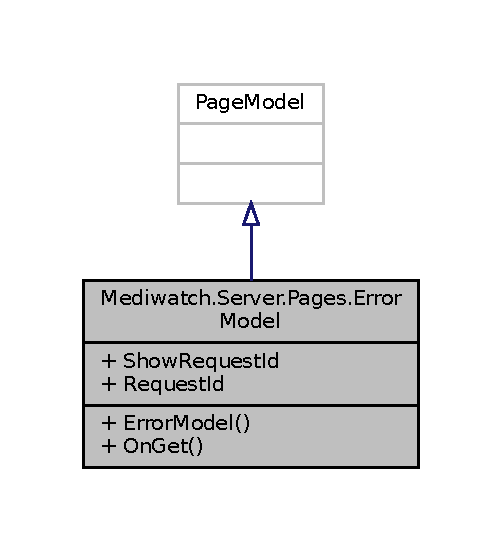
\includegraphics[width=241pt]{class_mediwatch_1_1_server_1_1_pages_1_1_error_model__inherit__graph}
\end{center}
\end{figure}


Graphe de collaboration de Mediwatch.\+Server.\+Pages.\+Error\+Model\+:\nopagebreak
\begin{figure}[H]
\begin{center}
\leavevmode
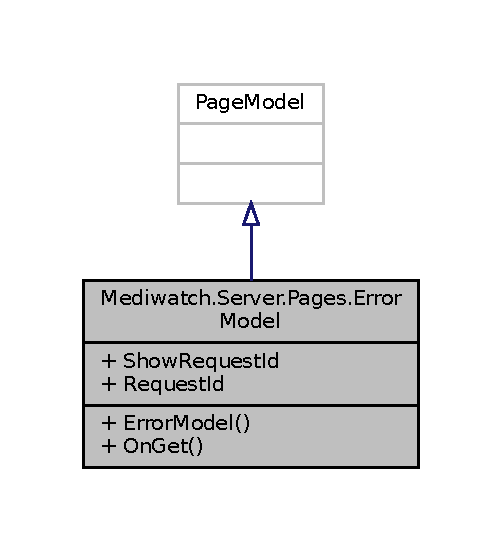
\includegraphics[width=241pt]{class_mediwatch_1_1_server_1_1_pages_1_1_error_model__coll__graph}
\end{center}
\end{figure}
\doxysubsection*{Fonctions membres publiques}
\begin{DoxyCompactItemize}
\item 
\mbox{\Hypertarget{class_mediwatch_1_1_server_1_1_pages_1_1_error_model_a6071f8072c63f30c32dac09a811f9ab3}\label{class_mediwatch_1_1_server_1_1_pages_1_1_error_model_a6071f8072c63f30c32dac09a811f9ab3}} 
{\bfseries Error\+Model} (I\+Logger$<$ \mbox{\hyperlink{class_mediwatch_1_1_server_1_1_pages_1_1_error_model}{Error\+Model}} $>$ logger)
\item 
\mbox{\Hypertarget{class_mediwatch_1_1_server_1_1_pages_1_1_error_model_afff141d7facfcb25a4a05e433cb18369}\label{class_mediwatch_1_1_server_1_1_pages_1_1_error_model_afff141d7facfcb25a4a05e433cb18369}} 
void {\bfseries On\+Get} ()
\end{DoxyCompactItemize}
\doxysubsection*{Attributs publics}
\begin{DoxyCompactItemize}
\item 
\mbox{\Hypertarget{class_mediwatch_1_1_server_1_1_pages_1_1_error_model_a63bd289fd620d1418adcd60cc4ff7f53}\label{class_mediwatch_1_1_server_1_1_pages_1_1_error_model_a63bd289fd620d1418adcd60cc4ff7f53}} 
bool {\bfseries Show\+Request\+Id} =$>$ !string.\+Is\+Null\+Or\+Empty(Request\+Id)
\end{DoxyCompactItemize}
\doxysubsection*{Propriétés}
\begin{DoxyCompactItemize}
\item 
\mbox{\Hypertarget{class_mediwatch_1_1_server_1_1_pages_1_1_error_model_a6b1ab7a6328fa0b58ac9b76c0d8bfbef}\label{class_mediwatch_1_1_server_1_1_pages_1_1_error_model_a6b1ab7a6328fa0b58ac9b76c0d8bfbef}} 
string {\bfseries Request\+Id}\hspace{0.3cm}{\ttfamily  \mbox{[}get, set\mbox{]}}
\end{DoxyCompactItemize}


La documentation de cette classe a été générée à partir du fichier suivant \+:\begin{DoxyCompactItemize}
\item 
Server/\+Pages/Error.\+cshtml.\+cs\end{DoxyCompactItemize}

\hypertarget{class_mediwatch_1_1_server_1_1_program}{}\doxysection{Référence de la classe Mediwatch.\+Server.\+Program}
\label{class_mediwatch_1_1_server_1_1_program}\index{Mediwatch.Server.Program@{Mediwatch.Server.Program}}


Graphe de collaboration de Mediwatch.\+Server.\+Program\+:
% FIG 0
\doxysubsection*{Fonctions membres publiques statiques}
\begin{DoxyCompactItemize}
\item 
static void \mbox{\hyperlink{class_mediwatch_1_1_server_1_1_program_a0b37e08654729aa1c9f3a572e5775305}{Main}} (string\mbox{[}$\,$\mbox{]} args)
\item 
static I\+Host\+Builder \mbox{\hyperlink{class_mediwatch_1_1_server_1_1_program_a5278302328dd5740238221820ef8fa07}{Create\+Host\+Builder}} (string\mbox{[}$\,$\mbox{]} args)
\end{DoxyCompactItemize}


\doxysubsection{Documentation des fonctions membres}
\mbox{\Hypertarget{class_mediwatch_1_1_server_1_1_program_a5278302328dd5740238221820ef8fa07}\label{class_mediwatch_1_1_server_1_1_program_a5278302328dd5740238221820ef8fa07}} 
\index{Mediwatch.Server.Program@{Mediwatch.Server.Program}!CreateHostBuilder@{CreateHostBuilder}}
\index{CreateHostBuilder@{CreateHostBuilder}!Mediwatch.Server.Program@{Mediwatch.Server.Program}}
\doxysubsubsection{\texorpdfstring{CreateHostBuilder()}{CreateHostBuilder()}}
{\footnotesize\ttfamily static I\+Host\+Builder Mediwatch.\+Server.\+Program.\+Create\+Host\+Builder (\begin{DoxyParamCaption}\item[{string\mbox{[}$\,$\mbox{]}}]{args }\end{DoxyParamCaption})\hspace{0.3cm}{\ttfamily [static]}}

\mbox{\Hypertarget{class_mediwatch_1_1_server_1_1_program_a0b37e08654729aa1c9f3a572e5775305}\label{class_mediwatch_1_1_server_1_1_program_a0b37e08654729aa1c9f3a572e5775305}} 
\index{Mediwatch.Server.Program@{Mediwatch.Server.Program}!Main@{Main}}
\index{Main@{Main}!Mediwatch.Server.Program@{Mediwatch.Server.Program}}
\doxysubsubsection{\texorpdfstring{Main()}{Main()}}
{\footnotesize\ttfamily static void Mediwatch.\+Server.\+Program.\+Main (\begin{DoxyParamCaption}\item[{string\mbox{[}$\,$\mbox{]}}]{args }\end{DoxyParamCaption})\hspace{0.3cm}{\ttfamily [static]}}



La documentation de cette classe a été générée à partir du fichier suivant \+:\begin{DoxyCompactItemize}
\item 
Server/\mbox{\hyperlink{_program_8cs}{Program.\+cs}}\end{DoxyCompactItemize}

\hypertarget{class_mediwatch_1_1_server_1_1_startup}{}\section{Référence de la classe Mediwatch.\+Server.\+Startup}
\label{class_mediwatch_1_1_server_1_1_startup}\index{Mediwatch.\+Server.\+Startup@{Mediwatch.\+Server.\+Startup}}


Graphe de collaboration de Mediwatch.\+Server.\+Startup\+:
\nopagebreak
\begin{figure}[H]
\begin{center}
\leavevmode
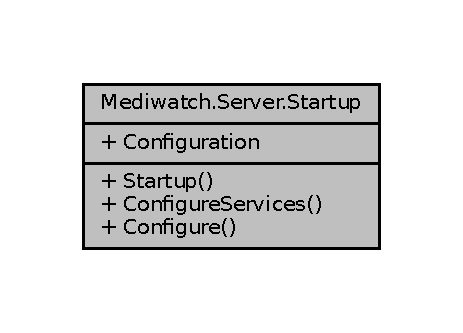
\includegraphics[width=210pt]{class_mediwatch_1_1_server_1_1_startup__coll__graph}
\end{center}
\end{figure}
\subsection*{Fonctions membres publiques}
\begin{DoxyCompactItemize}
\item 
\mbox{\Hypertarget{class_mediwatch_1_1_server_1_1_startup_a99779cbd7c184cbff98730a5f285a647}\label{class_mediwatch_1_1_server_1_1_startup_a99779cbd7c184cbff98730a5f285a647}} 
{\bfseries Startup} (I\+Configuration configuration)
\item 
\mbox{\Hypertarget{class_mediwatch_1_1_server_1_1_startup_a98b7f4b5e49a83c353687ec3c1cfa139}\label{class_mediwatch_1_1_server_1_1_startup_a98b7f4b5e49a83c353687ec3c1cfa139}} 
void {\bfseries Configure\+Services} (I\+Service\+Collection services)
\item 
\mbox{\Hypertarget{class_mediwatch_1_1_server_1_1_startup_af31b63124f79f812e79cb6f43df14a40}\label{class_mediwatch_1_1_server_1_1_startup_af31b63124f79f812e79cb6f43df14a40}} 
void {\bfseries Configure} (I\+Application\+Builder app, I\+Web\+Host\+Environment env)
\end{DoxyCompactItemize}
\subsection*{Propriétés}
\begin{DoxyCompactItemize}
\item 
\mbox{\Hypertarget{class_mediwatch_1_1_server_1_1_startup_ae3d0512feacc2872ab0ec4d5082626a6}\label{class_mediwatch_1_1_server_1_1_startup_ae3d0512feacc2872ab0ec4d5082626a6}} 
I\+Configuration {\bfseries Configuration}\hspace{0.3cm}{\ttfamily  \mbox{[}get\mbox{]}}
\end{DoxyCompactItemize}


La documentation de cette classe a été générée à partir du fichier suivant \+:\begin{DoxyCompactItemize}
\item 
Server/Startup.\+cs\end{DoxyCompactItemize}

\hypertarget{class_mediwatch_1_1_server_1_1_controllers_1_1_weather_forecast_controller}{}\doxysection{Référence de la classe Mediwatch.\+Server.\+Controllers.\+Weather\+Forecast\+Controller}
\label{class_mediwatch_1_1_server_1_1_controllers_1_1_weather_forecast_controller}\index{Mediwatch.Server.Controllers.WeatherForecastController@{Mediwatch.Server.Controllers.WeatherForecastController}}


Graphe d\textquotesingle{}héritage de Mediwatch.\+Server.\+Controllers.\+Weather\+Forecast\+Controller\+:
\nopagebreak
\begin{figure}[H]
\begin{center}
\leavevmode
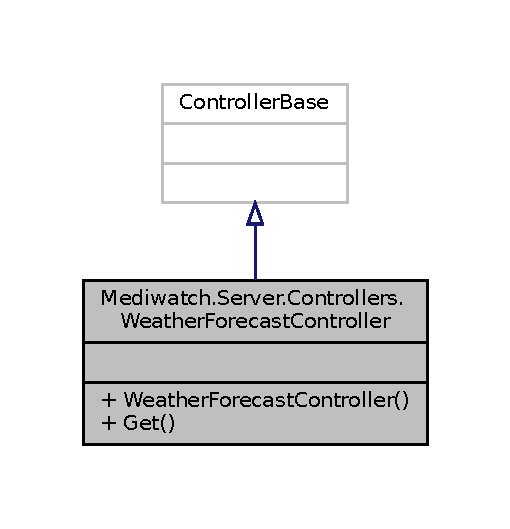
\includegraphics[width=245pt]{class_mediwatch_1_1_server_1_1_controllers_1_1_weather_forecast_controller__inherit__graph}
\end{center}
\end{figure}


Graphe de collaboration de Mediwatch.\+Server.\+Controllers.\+Weather\+Forecast\+Controller\+:
\nopagebreak
\begin{figure}[H]
\begin{center}
\leavevmode
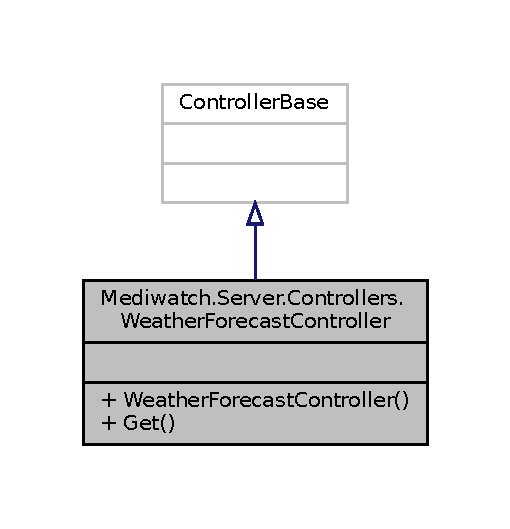
\includegraphics[width=245pt]{class_mediwatch_1_1_server_1_1_controllers_1_1_weather_forecast_controller__coll__graph}
\end{center}
\end{figure}
\doxysubsection*{Fonctions membres publiques}
\begin{DoxyCompactItemize}
\item 
\mbox{\Hypertarget{class_mediwatch_1_1_server_1_1_controllers_1_1_weather_forecast_controller_a8557f93a28d98c9487aa7c812cb61c18}\label{class_mediwatch_1_1_server_1_1_controllers_1_1_weather_forecast_controller_a8557f93a28d98c9487aa7c812cb61c18}} 
{\bfseries Weather\+Forecast\+Controller} (I\+Logger$<$ \mbox{\hyperlink{class_mediwatch_1_1_server_1_1_controllers_1_1_weather_forecast_controller}{Weather\+Forecast\+Controller}} $>$ logger)
\item 
\mbox{\Hypertarget{class_mediwatch_1_1_server_1_1_controllers_1_1_weather_forecast_controller_a43eaa75ecf6f43cba687aeb38a08636f}\label{class_mediwatch_1_1_server_1_1_controllers_1_1_weather_forecast_controller_a43eaa75ecf6f43cba687aeb38a08636f}} 
I\+Enumerable$<$ Weather\+Forecast $>$ {\bfseries Get} ()
\end{DoxyCompactItemize}


La documentation de cette classe a été générée à partir du fichier suivant \+:\begin{DoxyCompactItemize}
\item 
Server/\+Controllers/Weather\+Forecast\+Controller.\+cs\end{DoxyCompactItemize}

%--- End generated contents ---

% Index
\backmatter
\newpage
\phantomsection
\clearemptydoublepage
\addcontentsline{toc}{chapter}{Index}
\printindex

\end{document}
